\documentclass[../main.tex]{subfiles}

\begin{document}
\section{Offerta e forme di mercato}

Una decisione fondamentale per le imprese è definire la \textbf{quantità q di un bene da produrre per massimizzare il profitto} $\pi$, definito come:
$$\pi(q) = RT(q) - CT(q)$$
Per trovare il massimo in funzione della quantità q, si calcola la derivata prima e si uguaglia a 0:
$$\max_q \pi = \frac{\partial \pi(q)}{\partial q}=RM(q) - CM(q) = 0$$
$$\mathbf{RM(q) = CM(q)}$$
\begin{itemize}
    \item $\mathbf{RM(q)}$ \textbf{ricavo marginale}: derivata prima del ricavo, rappresenta il ricavo ottenuto servendo un cliente aggiuntivo.
    \item $\mathbf{CM(q)}$ \textbf{costo marginale}: derivata prima del cost, rappresenta il corso di servire un cliente aggiuntivo.
\end{itemize}

L'impresa considera di servire un cliente in più solo se effettivamente servire quel cliente aggiuntivo genera profitti addizionali, e non rappresenta un costo marginale maggiore del ricavo marginale.

La capacità delle imprese di massimizzare il profitto dipende da \textbf{fattori di mercato} quali
\begin{itemize}
    \item \textbf{Numero di concorrenti} (imprese che producono beni che i consumatori percepiscono come stretti sostituti).
    \item \textbf{Natura del prodotto} (omogeneo vs. differenziato).
    \item \textbf{Grado di libertà di entrata} (o uscita) delle imprese nel mercato.
    \item \textbf{Quantità dell'informazione} detenuta da imprese e consumatori.
    \item \dots
\end{itemize}

Tali caratteristiche definiscono la \textbf{forma di mercato (livello di competizione)} in cui opera l'impresa.

I mercati si collocano in un continuum tra concorrenza perfetta e monopolio
\begin{itemize}
    \item \textbf{Concorrenza perfetta}: infinite imprese nell'azienda, massimo livello di competizione.
    \item \textbf{Monopolio}: una sola impresa nell'industria, minimo livello di competizione.
\end{itemize}

\subsection{Concorrenza perfetta}

Il modello di concorrenza perfetta si basa su \textbf{quattro ipotesi fondamentali}.
\begin{enumerate}
    \item Esiste un \textbf{numero molto elevato di imprese} nel mercato; la singola impresa produce una quota trascurabile dell'offerta totale.
    \item Tutte le imprese producono un \textbf{prodotto identico}; in altre parole, il prodotto è omogeneo (non differenziato).
    \item Acquirenti e venditori hanno una \textbf{conoscenza perfetta} dei prodotti e dei prezzi.
    \item Esiste \textbf{completa libertà di entrata e di uscita} da parte di nuove imprese.
\end{enumerate}

Non esiste un mercato che soddisfa perfettamente le condizioni elencate sopra, ma ci sono esempi che si avvicinano: \emph{mercato ortofrutticolo}, molti produttori, i prodotti venduti sono tutti gli stessi. Queste attività non sono particolarmente lucrative, fare profitti elevati è difficile.

La concorrenza perfetta è una \textbf{forma di mercato estrema}:
\begin{itemize}
    \item Le imprese non hanno alcun potere di influenzare il prezzo del prodotto.
    \item Il prezzo a cui vendono è determinato dall'interazione della domanda e dell'offerta complessiva di mercato (si veda dopo).
\end{itemize}

In altri termini le \textbf{imprese sono price-taker}
\begin{itemize}
    \item Se fissassero un \textbf{prezzo superiore} a quello di mercato, \textbf{non venderebbero nulla}.
    \item Se fissassero un \textbf{prezzo inferiore} a quello di mercato, \textbf{non avrebbero la capacità di soddisfare l'intero mercato}. Gli altri produttori continuano a vendere al loro prezzo e fanno più soldi, quindi non conviene.
\end{itemize}

\textbf{Qual è la quantità q che consente all'impresa di massimizzare il profitto (= ricavi - costi)?}

\subsubsection{Curva di offerta individuale}
La curva di offerta individuale esprime, \textbf{per ogni livello di prezzo p, la quantità ottimale q di produzione del bene}.

\begin{figure}[h]
    \centering
    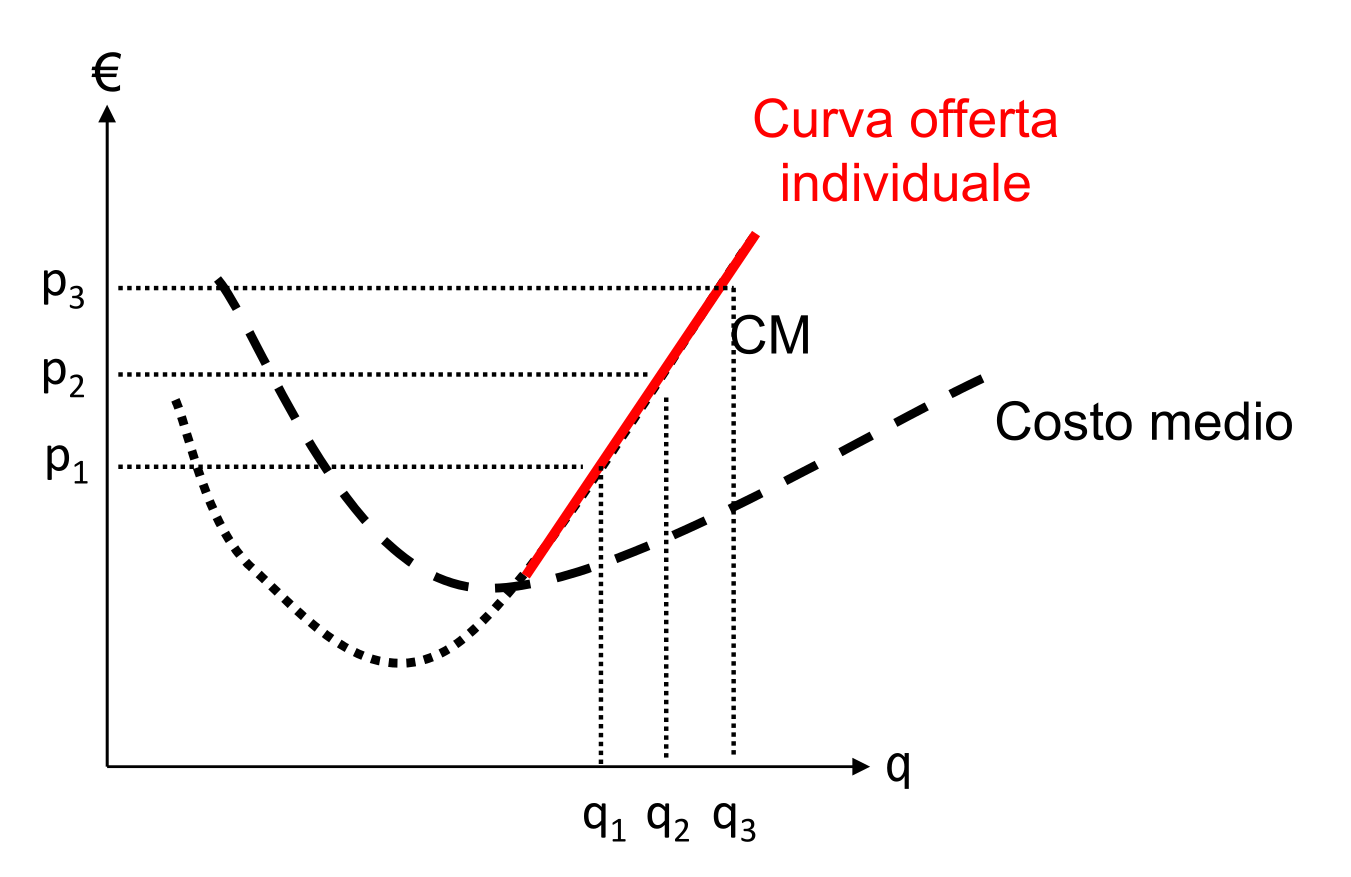
\includegraphics[width=0.8\textwidth]{curva-offerta-individuale.png}
\end{figure}

Essendo l'impresa price-taker, p non dipende dalla quantità prodotta dalla singola impresa q:
$$RT(q) = p\cdot q$$
$$RM(q) = p$$

\textbf{Condizione di massimizzazione del profitto}: $RM(q) = CM(q)$. Si ottiene quindi:
$$p = CM(q)$$

\textbf{Condizione minima di produzione}: $\pi = pq - CT(q) > 0$.

Si ottiene quindi che il prezzo deve essere superiore al costo medio affinchè l'impresa sia in grado di ottenere profitti positivi.
$$\mathbf{p > \frac{CT(q)}{q}}$$

\subsubsection{Curva di offerta di mercato}
La curva di offerta di mercato è la somma delle curve di offerta di tutte le imprese nel mercato.

\begin{figure}[h]
    \centering
    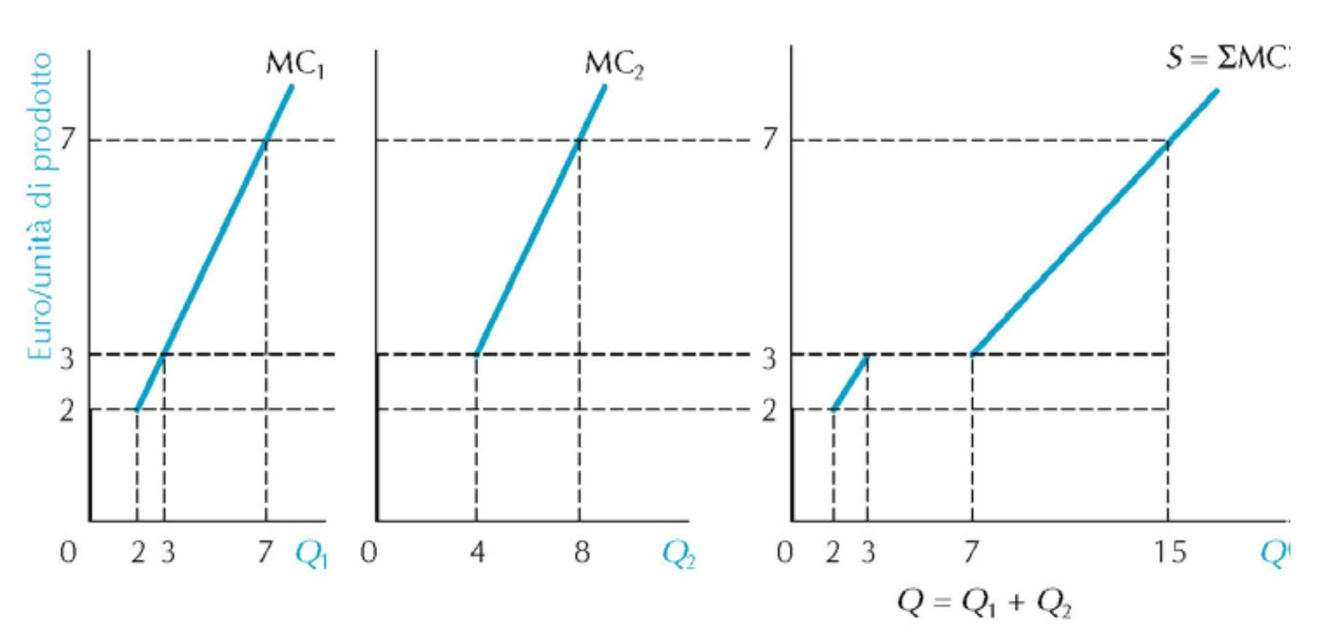
\includegraphics[width=0.95\textwidth]{curva-offerta-mercato.png}
\end{figure}

Se in un mercato in cui operano molteplici aziende produttrici, il \textbf{prezzo di equilibrio} dipende dall'\textbf{incontro tra domanda e offerta di mercato}.

\begin{itemize}
    \item \textbf{Se p $>$ prezzo di equilibrio di mercato} si verifica un \textbf{eccesso di offerta}, ovvero alcuni produttori non riescono a vendere. Di conseguenza il prezzo si abbassa per vendere di più, anche ai consumatori con prezzo di riserva più basso.
    \item \textbf{Se p $<$ prezzo di equilibrio di mercato} si verifica un \textbf{eccesso di domanda}, ovvero alcuni consumatori sarebbero disposti a comprare il bene ma questo non sarebbe disponibile.
\end{itemize}

Nel lungo periodo, se le imprese già operative ottengono profitti positivi (p $>$ costo medio), \textbf{nuove imprese saranno attirate nel mercato}.

La dinamica del prezzo nel mercato ha quindi un \textbf{andamento ciclico}:

\begin{itemize}
    \item nuove imprese entrano nel mercato attratte dal profitto.
    \item l'offerta sale e il prezzo di equilibrio scende.
    \item per alcune imprese diviene p $<$ costo medio.
    \item le imprese con costo medio $>$ p escono dal mercato.
    \item l'offerta scende e il prezzo sale
    \item \dots e così via.
\end{itemize}

\textbf{Equilibrio di lungo periodo}: entrata e uscita cessano quando non sono più possibili profitti. Rimangono sul mercato solo le imprese più efficienti che producono al costo medio minimo. Le \textbf{imprese conseguono profitti nulli}.

\textbf{Dal punto di vista dell'impresa, la concorrenza non è desiderabile.}

\subsection{Monopolio}

A volte in un mercato c'è un'\textbf{unica impresa produttrice} (monopolista).
Questo si verifica nel caso in cui esistono ostacoli insormontabili (le barriere all'entrata) che impediscono ad altre imprese di entrare e competere.

Il monopolista è \textbf{price-maker}:
\begin{itemize}
    \item A differenza della concorrenza perfetta, \textbf{fronteggia l'intera curva di domanda di mercato}.
    \item \textbf{Il prezzo al quale egli vende il prodotto non è indipendente dalla quantità venduta.}
\end{itemize}

Ne consegue che i ricavi totali sono dati da:
$$RT(q) = p(q)\cdot q$$
Ed il ricavo marginale è quindi:
$$
    RM(q)=\frac{\partial p(q)}{\partial q}\cdot q + p(q) = p(q)\cdot \left(\frac{\partial p(q)}{\partial q}\frac{q}{p(q)}+1\right)=p(q)\cdot \left(-\frac{1}{\varepsilon}+1\right)
$$
Dove $\varepsilon$ è l'elasticità della domanda al prezzo (in valore assoluto).

Si applica la \textbf{condizione di massimizzazione del profitto}: $RM(q) = CM(q)$, e si ottiene quindi
$$p(q)\cdot \left(-\frac{1}{\varepsilon}+1\right)=CM(q)$$
$$\mathbf{\frac{p(q)-CM(q)}{p(q)} = \frac{1}{\bm\varepsilon}}$$

Il monopolista fissa un prezzo al di sopra dei costi marginali (si dice che ha \textbf{potere di mercato}). Il potere di mercato è tanto maggiore quanto meno la domanda risponde alle variazioni di prezzo (ovvero se la domanda ha elasticità bassa).

\textbf{Per i consumatori è un bene? NO!}
\begin{itemize}
    \item Rispetto alla concorrenza perfetta, in monopolio si produce una quantità minore ad un prezzo maggiore.
    \item Ciò determina la \textbf{perdita secca di monopolio}: perdita di surplus dei consumatori del quale non si appropria il monopolista (inefficienza allocativa).
\end{itemize}

\subsubsection{Intervento dello Stato}

Lo stato può intervenire con \textbf{leggi antitrust} per \textbf{stimolare la concorrenza}:
\begin{itemize}
    \item Impedire/approvare fusioni.
    \item Frazionare imprese divenute troppo grandi.
    \item Impedire comportamenti volti a ridurre la concorrenza.
\end{itemize}

Alternativamente può attuare una \textbf{regolamentazione}, ovvero:
\begin{itemize}
    \item Imporre al monopolista di offrire il bene a $p = CM$.
\end{itemize}

Si può anche attuare una \textbf{trasformazione dei monopoli privati in imprese pubbliche}:
\begin{itemize}
    \item Lo Stato si fa imprenditore e gestisce direttamente la produzione.
    \item Rischi:
          \begin{itemize}
              \item Riduzione dell'efficienza produttiva
              \item Logiche clientelari.
          \end{itemize}
\end{itemize}

\subsubsection{Nascita del monopolio}

Il monopolio è \textbf{generato dalle barriere all'entrata}, che possono essere di vari tipi:
\begin{itemize}
    \item \textbf{Istituzionali}: barriere poste dallo Stato stesso, come ad esempio licenze e permessi, o brevetti.

          Queste potrebbero essere introdotte per motivi di efficienza produttiva (non conviene che sul mercato operino due aziende).
    \item \textbf{Strutturali}: ovvero che dipendono da caratteristiche di tecnologia e domanda e rendono l'entrata molto costosa.
          \begin{itemize}
              \item \textbf{Vantaggi di costo} delle imprese che sono già sul mercato: proprietà di risorse scarse, maggiore efficienza dovuta a processi di apprendimento, migliori legami coi fornitori e istituzioni finanziarie.
              \item \textbf{Economie di scala}: al crescere di q, si riducono i costi medi. Un nuovo arrivato ci mette un po' di tempo per arrivare ad una condizione di efficienza.
          \end{itemize}
    \item \textbf{Strategiche}: sono messe in atto dalle imprese già presenti sul mercato per inibire l'entrata di potenziali rivali, o indurre l'uscita dei nuovi concorrenti, una volta che l'entrata è avvenuta.

          Esempio: \textbf{prezzi predatori}, ovvero prezzi minori del costo marginale praticati temporaneamente per danneggiare i nuovi concorrenti ed indurli ad uscire dal mercato.
\end{itemize}

\end{document}